\section{LASSO}
%%%%%%%%%%%%%%%%%%%%%%%%%%%%%%%%%%%%%%%%%%%%%%%%%%%%%%%%
\begin{frame}
  \frametitle{Least Absolute Shrinkage and Selection Operator (LASSO)}
  \framesubtitle{B\"{u}hlmann \& van de Geer (2011); Hastie, Tibshirani \& Wainwright (2015)}

  Assume that $X$ has been centered: don't penalize intercept!

  \begin{block}{Notation}
    $\left| \left| \beta\right| \right|_2^2 = \sum_{j=1}^p \beta_j^2, \quad \left| \left| \beta\right| \right|_1 = \sum_{j=1}^p |\beta_j|$
  \end{block}

  \begin{block}{Ridge Regression -- $L_2$ Penalty}
	$\widehat{\beta}_{Ridge} =\underset{\beta}{\arg \min}\; (\mathbf{y} -  X\beta)' (\mathbf{y} - X\beta) + \lambda \left| \left| \beta\right| \right|_2^2$
  \end{block}

  \begin{block}{LASSO -- $L_1$ Penalty}
	$\widehat{\beta}_{Lasso} =\underset{\beta}{\arg \min}\; (\mathbf{y} - X\beta)' (\mathbf{y} - X\beta) + \lambda \left| \left| \beta\right| \right|_1$
  \end{block}

  
\end{frame}
%%%%%%%%%%%%%%%%%%%%%%%%%%%%%%%%%%%%%%%%%%%%%%%%%%%%%%%%
\begin{frame}
  \frametitle{Other Ways of Thinking about LASSO}
  \begin{block}{Constrained Optimization}
	$\underset{\beta}{\arg \min} (\mathbf{y}  - X\beta)' (\mathbf{y} - X\beta) \quad \mbox{subject to}\quad \sum_{j=1}^p |\beta_j| \leq t$
Data-dependent, one-to-one mapping between $\lambda$ and $t$.
\end{block}

\begin{block}{Bayesian Posterior Mode}
    Ignoring the intercept, LASSO is the posterior model for $\beta$ under
		\[\mathbf{y}|X,\beta, \sigma^2 \sim N(X\beta,\sigma^2 I_n), \quad
    \beta\sim \prod_{j=1}^p \mbox{Lap}(\beta_j|0, \tau)\]
  where  
  $\lambda= 1/\tau$ and 
  $\mbox{Lap}(x|\mu,\tau)= (2\tau)^{-1}\exp\left \{-\tau^{-1}|x-\mu| \right\}$
\end{block}
\end{frame}
%%%%%%%%%%%%%%%%%%%%%%%%%%%%%%%%%%%%%%%%%%%%%%%%%%%%%%%%
\begin{frame}
  \frametitle{Comparing Ridge and LASSO -- Bayesian Posterior Modes}
    
\begin{figure}
	\centering
	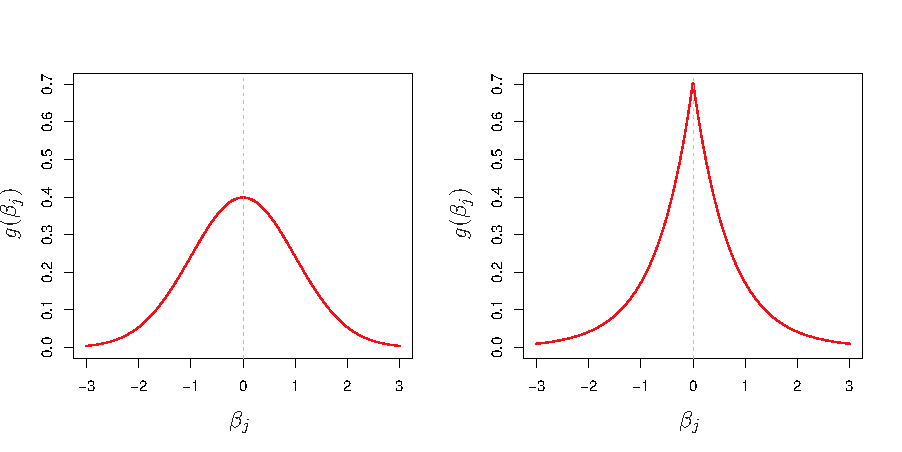
\includegraphics[scale=0.65]{../img/ISLR_ch6_fig11}
	\label{fig:ridge_lasso_prior}
  \caption{Ridge, at left, puts a normal prior on $\beta$ while LASSO, at right, uses a Laplace prior, which has fatter tails and a taller peak at zero.}
\end{figure}

\end{frame}
%%%%%%%%%%%%%%%%%%%%%%%%%%%%%%%%%%%%%%%%%%%%%%%%%%%%%%%%
\begin{frame}
  \frametitle{Comparing LASSO and Ridge -- Constrained OLS}
  
\begin{figure}
	\centering
	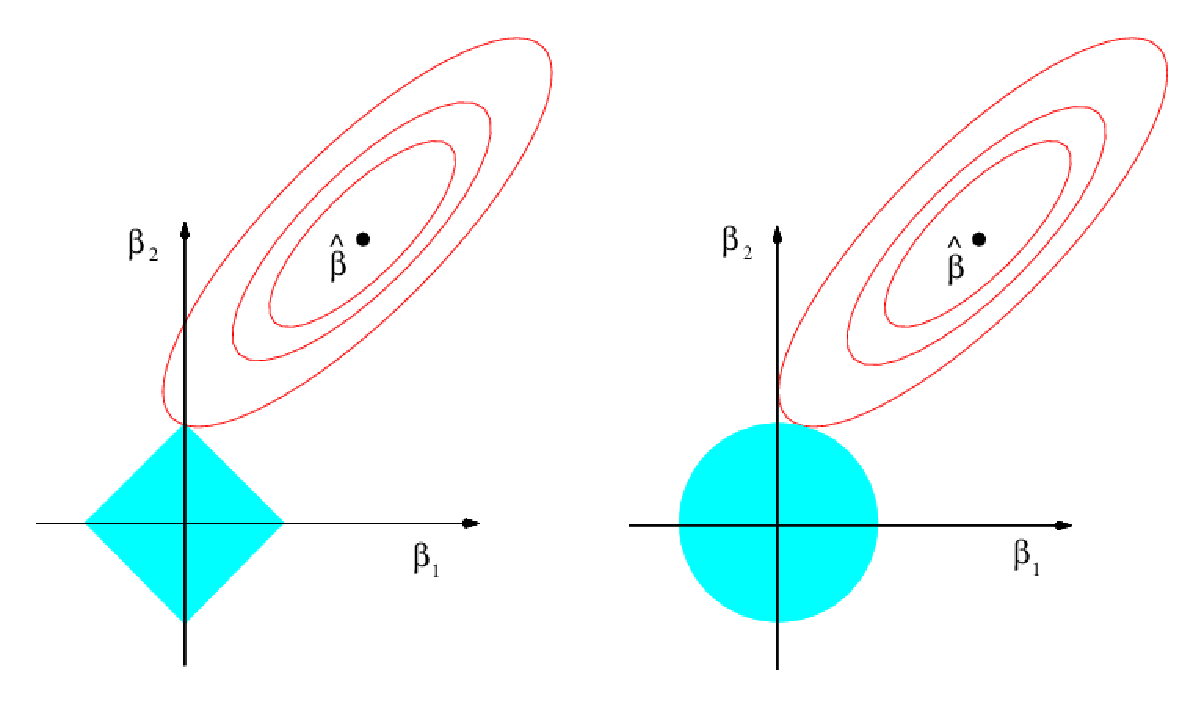
\includegraphics[scale=0.4]{../img/ISLR_ch6_fig7}
	\caption{$\widehat{\beta}$ denotes the MLE and the ellipses are the contours of the likelihood. 
LASSO, at left, and Ridge, at right, both shrink $\beta$ away from the MLE towards zero.
Because of its diamond-shaped constraint set, however, LASSO favors a \alert{sparse solution} while Ridge does not}
	\label{fig:ridge_lasso_constraint}
\end{figure}
\end{frame}
%%%%%%%%%%%%%%%%%%%%%%%%%%%%%%%%%%%%%%%%%%%%%%%%%%%%%%%%
